% !TeX program = xelatex
\documentclass[a4paper,10pt]{article}

% ============================================================================
% សន្លឹកកិច្ចការសិស្សបំពេញចន្លោះ ស-ខ្មៅ និងប្លង់ក្ដារខៀន/ចម្លើយគ្រូ (គ្មាន LCD / គ្មានកន្ត្រៃ)
% មេរៀនទី៦ (៣)៖ ការសម្រួលកន្សោមសនិទាន — ត្រូវគ្នានឹង LS_Plan_RAT62.tex
% ============================================================================
\usepackage[a4paper, left=1.0cm, right=1.0cm, top=0.75cm, bottom=1.00cm, footskip=0.52cm]{geometry}
\usepackage{amsmath}
\usepackage{unicode-math}
\usepackage{fontspec}
\usepackage{array, colortbl}
\usepackage[table]{xcolor}
\usepackage{enumitem}
\usepackage{pifont}
\usepackage{fancyhdr}
\usepackage{lastpage}
\usepackage{tikz}
\usepackage[most]{tcolorbox}
\usetikzlibrary{calc, arrows.meta, decorations.pathreplacing, positioning, babel}

\makeatletter
\let\@expl@@@mark@update@singlecol@structures@@\relax
\makeatother

\providecommand{\NGSFindFonts}{%
  \IfFileExists{C:/Windows/Fonts/cambria.ttc}{%
    \def\NGSSysPath{C:/Windows/Fonts/}%
    \def\NGSUserPath{C:/Users/KIT/AppData/Local/Microsoft/Windows/Fonts/}%
  }{%
    \IfFileExists{./fonts/KhmerOSsiemreap.ttf}{\def\NGSSysPath{./fonts/}\def\NGSUserPath{./fonts/}}{%
    \IfFileExists{../fonts/KhmerOSsiemreap.ttf}{\def\NGSSysPath{../fonts/}\def\NGSUserPath{../fonts/}}{%
    \IfFileExists{../../fonts/KhmerOSsiemreap.ttf}{\def\NGSSysPath{../../fonts/}\def\NGSUserPath{../../fonts/}}{%
    \IfFileExists{../../../fonts/KhmerOSsiemreap.ttf}{\def\NGSSysPath{../../../fonts/}\def\NGSUserPath{../../../fonts/}}{%
    \IfFileExists{../../../../fonts/KhmerOSsiemreap.ttf}{\def\NGSSysPath{../../../../fonts/}\def\NGSUserPath{../../../../fonts/}}{%
    \IfFileExists{../../../../../fonts/KhmerOSsiemreap.ttf}{\def\NGSSysPath{../../../../../fonts/}\def\NGSUserPath{../../../../../fonts/}}{%
    \IfFileExists{../../../../../../fonts/KhmerOSsiemreap.ttf}{\def\NGSSysPath{../../../../../../fonts/}\def\NGSUserPath{../../../../../../fonts/}}{%
      \def\NGSSysPath{../../../../../../../fonts/}\def\NGSUserPath{../../../../../../../fonts/}%
    }}}}}}}%
  }%
}
\NGSFindFonts

\setmathfont[Path={\NGSSysPath}, FontIndex=1, Scale=1.02]{cambria.ttc}
\defaultfontfeatures{Ligatures=TeX}

\setmainfont[
  Path={\NGSUserPath}, Extension=.ttf, Script=Khmer,
  BoldFont={KhmerOSsiemreap}, BoldFeatures={FakeBold=1.8},
  ItalicFont={KhmerOSsiemreap}, ItalicFeatures={FakeSlant=0.25},
  BoldItalicFont={KhmerOSsiemreap}, BoldItalicFeatures={FakeBold=1.8, FakeSlant=0.25}
]{KhmerOSsiemreap}

\newfontfamily\muol[Path={\NGSUserPath}, Extension=.ttf, Script=Khmer]{KhmerOSmuollight}
\newfontfamily\TimesEn[Path={\NGSSysPath}, Extension=.ttf, BoldFont={timesbd}, ItalicFont={timesi}, BoldItalicFont={timesbi}]{times}
\newfontfamily\CalibriFont[Path={\NGSSysPath}, Extension=.ttf]{calibri}

\XeTeXlinebreaklocale "km"
\XeTeXlinebreakskip = 0pt plus 1pt minus 0.1pt

\definecolor{panelgray}{gray}{0.94}
\definecolor{headgray}{gray}{0.85}

\pagestyle{fancy}
\fancyhf{}
\renewcommand{\headrulewidth}{0pt}
\fancyfoot[L]{\fontsize{7.4pt}{9.5pt}\selectfont អនុវិទ្យាល័យព្រះក្រសាំង \en{|} គ្រូ៖ ហុក ប៊ុនថែន \en{|} មេរៀនទី៦ (៣) ការសម្រួលកន្សោមសនិទាន \en{|} ថ្ងៃអង្គារ ទី១៥ ខែធ្នូ ឆ្នាំ២០២៦}
\fancyfoot[R]{\fontsize{7.8pt}{10pt}\selectfont ទំព័រ \en{\thepage\ / \pageref{LastPage}}}

\setlength{\parindent}{0pt}
\setlength{\parskip}{0pt}
\setlength{\tabcolsep}{4pt}

\newcommand{\en}[1]{{\TimesEn #1}}
\newcommand{\enbf}[1]{{\TimesEn\bfseries #1}}
\newcommand{\unit}[1]{\,\text{\en{#1}}}
\newcommand{\riel}{\,\text{៛}}
\newcommand{\cnum}[1]{\mbox{\fontsize{10pt}{12pt}\selectfont\ding{\numexpr181+#1\relax}}}
\newcommand{\chkbox}{\tikz[baseline=-0.15ex]\draw[black, line width=0.85pt, fill=white] (0,0) rectangle (0.24cm,0.24cm);}
\newcommand{\ansbox}[1][2.0cm]{\,\tikz[baseline=-0.65ex]\draw[black, line width=0.65pt, fill=white] (0,0) rectangle (#1, 0.42cm);\,}
\newcommand{\dotline}[1][2.2cm]{\makebox[#1]{\dotfill}}

\newcommand{\pagebanner}[2]{%
  \begin{tcolorbox}[
    enhanced, sharp corners, colback=headgray, colframe=black,
    boxrule=1.05pt, boxsep=1pt, top=2.5pt, bottom=2.5pt, left=6pt, right=6pt,
    after skip=3.5pt
  ]
    {\muol\fontsize{9.0pt}{13.2pt}\selectfont #1}\hfill{\fontsize{8.0pt}{11.2pt}\selectfont\textbf{#2}}
  \end{tcolorbox}%
}

\newcommand{\secstrip}[2]{%
  \vspace{3pt}%
  \begin{tcolorbox}[
    enhanced, sharp corners, colback=panelgray, colframe=black,
    boxrule=0.8pt, boxsep=0.8pt, top=2pt, bottom=2pt, left=5pt, right=5pt,
    after skip=3pt
  ]
    {\muol\fontsize{8.5pt}{12.2pt}\selectfont #1}\hfill{\fontsize{7.8pt}{10.8pt}\selectfont\textit{#2}}
  \end{tcolorbox}%
}

\newcolumntype{L}[1]{>{\raggedright\arraybackslash}p{#1}}
\newcolumntype{C}[1]{>{\centering\arraybackslash}p{#1}}

\begin{document}
\fontsize{9.5pt}{14.5pt}\selectfont

% ============================================================================
% ទំព័រទី ១៖ សន្លឹកកិច្ចការសិស្ស (ផ្នែកមុខ៖ E1 -> E2 -> E3)
% ============================================================================
\pagebanner{សន្លឹកកិច្ចការសិស្ស \enbf{(}៦\enbf{.}៣ ការសម្រួលកន្សោមសនិទាន\enbf{)} \enbf{--} ផ្នែកមុខ}{ថ្នាក់ទី៨ \en{|} ទំ.៧៦--៧៨}

\begin{tcolorbox}[
  enhanced, sharp corners, colback=white, colframe=black,
  boxrule=0.8pt, boxsep=1.5pt, top=3.5pt, bottom=3.5pt, left=5pt, right=5pt,
  after skip=4pt
]
  \fontsize{9.0pt}{13.0pt}\selectfont
  \textbf{ឈ្មោះសិស្ស៖} \dotline[4.3cm] \quad
  \textbf{សមាជិកក្រុម៖} \dotline[4.3cm] \quad
  \textbf{ថ្នាក់ទី៖} ៨\dotline[0.9cm] \quad
  \textbf{ក្រុមទី៖} \dotline[1.0cm]
\end{tcolorbox}

% --- E1 Engage ---
\secstrip{ផ្នែកទី ១ \enbf{(E1 - Engage)} ៖ បេសកកម្មចាប់កំហុសសម្រួលតួឆ្លងសញ្ញាបូក}{រយៈពេល ៣ នាទី (គូស \ding{51} ក្នុង \chkbox)}

\begin{tcolorbox}[
  enhanced, sharp corners, colback=white, colframe=black,
  boxrule=0.8pt, boxsep=2.5pt, top=4pt, bottom=4pt, left=6pt, right=6pt
]
  គេចង់សម្រួលកន្សោមសនិទាន $\dfrac{3x^2 + 4x}{9x^2 - 16}$ (ទំ.៧៧) ។ តើសិស្សរូបណាសម្រួលបានត្រឹមត្រូវ?\\[3pt]
  \chkbox\ \textbf{សិស្ស ក៖} ឈូត $x^2$ ឆ្លងបូក-ដក បាន $-\dfrac{3 + 4x}{7}$ \qquad
  \chkbox\ \textbf{សិស្ស ខ៖} ដាក់ជាកត្តា បាន $\dfrac{x(3x+4)}{(3x-4)(3x+4)} = \dfrac{x}{3x - 4}$\\[3pt]
  $\bullet$ \textbf{តេស្តដោយជំនួស $x = 2$៖} កន្សោមដើមស្មើ $\dfrac{20}{20} = 1$; \ ចម្លើយសិស្ស ក ស្មើ \ansbox[1.8cm]; \ សិស្ស ខ ស្មើ \ansbox[1.8cm] ។
\end{tcolorbox}

\vspace{3pt}

% --- E2 Explore ---
\secstrip{ផ្នែកទី ២ \enbf{(E2 - Explore)} ៖ សម្រួលតាមកត្តារួម សមភាពសំខាន់ៗ និងកត្តាផ្ទុយ (ទំ.៧៦--៧៧)}{រយៈពេល ១១ នាទី}

\textbf{សកម្មភាព ១ (\en{E2-A} — ៥ នាទី)៖ សម្រួលតាមកត្តារួម និងឯកធា (ទំ.៧៦--៧៧ ឧទាហរណ៍ទី ១ និងទី ២)}

\begin{tcolorbox}[
  enhanced, sharp corners, colback=white, colframe=black,
  boxrule=0.8pt, boxsep=2.5pt, top=4pt, bottom=4pt, left=6pt, right=6pt
]
  $\bullet$ \textbf{១) ឧទាហរណ៍ទី ១៖} $\dfrac{2x - 6}{5x - 15} = \dfrac{2(\phantom{x-3})}{5(\phantom{x-3})} \longrightarrow$ ចែកនឹងកត្តារួម $(x - 3)$ បាន \ansbox[2.4cm]\\[4pt]
  $\bullet$ \textbf{២) ឧទាហរណ៍ទី ២៖} $\dfrac{12a^2b^3}{15a^5b} = \dfrac{3a^2b \cdot 4b^2}{3a^2b \cdot 5a^3} \longrightarrow$ ចែកនឹងកត្តារួម $3a^2b$ បាន \ansbox[2.6cm]
\end{tcolorbox}

\vspace{4pt}
\textbf{សកម្មភាព ២ (\en{E2-B} — ៦ នាទី)៖ សមភាពសំខាន់ៗ និងកត្តាផ្ទុយ $1 - x = -(x - 1)$ (ទំ.៧៧ ឧទាហរណ៍ទី ៣ និងទី ៤)}

\begin{tcolorbox}[
  enhanced, sharp corners, colback=white, colframe=black,
  boxrule=0.8pt, boxsep=2.5pt, top=4pt, bottom=4pt, left=6pt, right=6pt
]
  $\bullet$ \textbf{១) ឧទាហរណ៍ទី ៣៖} $\dfrac{3x^2 + 4x}{9x^2 - 16} = \dfrac{x(3x + 4)}{(3x - 4)(3x + 4)} =$ \ansbox[3.2cm]\\[4pt]
  $\bullet$ \textbf{២) ឧទាហរណ៍ទី ៤ (កត្តាផ្ទុយ)៖} $\dfrac{1 - x}{x^2 + x - 2} = \dfrac{-(x - 1)}{(x - 1)(x + 2)} =$ \ansbox[3.2cm]
\end{tcolorbox}

\vfill

% --- E3 Explain ---
\secstrip{ផ្នែកទី ៣ \enbf{(E3 - Explain)} ៖ សង្ខេបវិធានសម្រួល និងធនាគារហេតុផល \enbf{B\&W}}{រយៈពេល ៦ នាទី}

\begin{tcolorbox}[
  enhanced, sharp corners, colback=white, colframe=black,
  boxrule=0.85pt, boxsep=2.5pt, top=4pt, bottom=4pt, left=6pt, right=6pt
]
  $\bullet$ \textbf{១) វិធានជាទូទៅ៖} ដាក់ភាគយកនិងភាគបែងជា \dotline[3.4cm] រួចចែកនឹងកត្តារួមខុសពីសូន្យ៖ $\dfrac{AK}{BK} =$ \ansbox[2.0cm]\\[4pt]
  $\bullet$ \textbf{២) លក្ខណៈកត្តាផ្ទុយ៖} ដោយ $b - a = -(a - b)$ គេបាន $\dfrac{b - a}{a - b} =$ \ansbox[2.0cm] ($a \neq b$)\\[4pt]
  \tikz\draw[black, dashed, line width=0.6pt] (0,0) -- (\linewidth,0);\\[3pt]
  \fontsize{8.8pt}{13.0pt}\selectfont
  \textbf{ធនាគារហេតុផល (\en{Warrant Bank})៖} \quad
  \cnum{1} ហាមឈូតតួឆ្លងសញ្ញា $(+)/(-)$ មុនដាក់ជាផលគុណកត្តា\\
  \cnum{2} សម្រួលបានតែកត្តារួមខុសពីសូន្យ ($K \neq 0$) \quad
  \cnum{3} កត្តាផ្ទុយ $\tfrac{b-a}{a-b} = -1$ \quad
  \cnum{4} សម្រួលអស់ពីភាគយកនៅសល់លេខ $1$
\end{tcolorbox}

% ============================================================================
% ទំព័រទី ២៖ សន្លឹកកិច្ចការសិស្ស (ផ្នែកខាងខ្នង៖ E4 -> E5 -> កិច្ចការផ្ទះ)
% ============================================================================
\clearpage
\pagebanner{សន្លឹកកិច្ចការសិស្ស \enbf{(}៦\enbf{.}៣ ការសម្រួលកន្សោមសនិទាន\enbf{)} \enbf{--} ផ្នែកខ្នង}{ថ្នាក់ទី៨ \en{|} ទំ.៧៨, ៨៥}

% --- E4 Elaborate ---
\secstrip{ផ្នែកទី ៤ \enbf{(E4 - Elaborate)} ៖ លំហាត់គំរូទី ១--២ និងប្រតិបត្តិ ក, ខ (ទំ.៧៨)}{រយៈពេល ១០ នាទី}

\begin{tcolorbox}[
  enhanced, sharp corners, colback=white, colframe=black,
  boxrule=0.8pt, boxsep=2.5pt, top=4pt, bottom=4pt, left=6pt, right=6pt
]
  \textbf{១) លំហាត់គំរូទី ១ និងទី ២ (ទំ.៧៨)៖}\\[3pt]
  \hspace*{0.3cm}$\bullet$ គំរូ ១៖ $\dfrac{(x-3)(3x-1)-(2x-6)(x+1)}{1-x^2} = \dfrac{(x-3)(x-1)}{-(x-1)(x+1)} =$ \ansbox[3.2cm]\\[3pt]
  \hspace*{0.3cm}$\bullet$ គំរូ ២ (រង្វង់ចារឹកក្នុងការេជ្រុង $x$ មានកាំ $\dfrac{x}{2}$)៖ ផលធៀបផ្ទៃរង្វង់និងការេគឺ $\dfrac{\frac{\pi}{4}x^2}{x^2} =$ \ansbox[2.2cm]\\[4pt]
  \textbf{២) ប្រតិបត្តិ ក, ខ (ទំ.៧៨)៖} ក) $\dfrac{a - b}{b^2 - a^2} =$ \ansbox[2.8cm] \quad
  ខ) $\dfrac{5(a-1) - a(a-1)}{5(a+2) - a^2 - 2a} =$ \ansbox[2.8cm]\\[4pt]
  \textbf{ឆ្លុះបញ្ចាំង (\en{EIA Looking-Back})៖} ហេតុអ្វីក្នុង $\dfrac{a - b}{b^2 - a^2}$ ក្រោយសម្រួល $(b-a)$ ភាគយកនៅសល់ $-1$? \dotline[3.4cm] ។
\end{tcolorbox}

\vspace{4pt}

% --- E5 Evaluate ---
\secstrip{ផ្នែកទី ៥ \enbf{(E5 - Evaluate)} ៖ ប្រតិបត្តិ (ទំ.៧៨, ៨៥) សំណួរវិនិច្ឆ័យ \enbf{A--D} និងសំបុត្រចេញ}{រយៈពេល ១០ នាទី}

\begin{tcolorbox}[
  enhanced, sharp corners, colback=white, colframe=black,
  boxrule=0.8pt, boxsep=2.5pt, top=4pt, bottom=4pt, left=6pt, right=6pt
]
  \textbf{១) ប្រតិបត្តិជាក្រុម (ទំ.៧៨ គ, ឃ និង ទំ.៨៥ \en{\#5})៖}\\[3pt]
  \hspace*{0.3cm}$\bullet$ ប្រតិបត្តិ គ៖ $\dfrac{x - y}{x^2 + xz - xy - zy} =$ \ansbox[2.6cm] \quad
  ប្រតិបត្តិ ឃ៖ $\dfrac{3a^3 - 3a^2 - 6a}{6a^3 - 12a^2 - 18a} =$ \ansbox[3.0cm]\\[3pt]
  \hspace*{0.3cm}$\bullet$ \en{\#5} ក៖ $\dfrac{14x^3}{7x^2y} =$ \ansbox[2.0cm] \quad
  \en{\#5} ឃ៖ $\dfrac{9ab(x-3)}{18a^2b(x^2-9)} =$ \ansbox[2.6cm] \quad
  \en{\#5} ច៖ $\dfrac{1 - 25x^2}{5x - 1} =$ \ansbox[2.4cm]\\[4pt]
  \textbf{២) បិទបេសកកម្ម \en{E1}៖} សិស្ស \dotline[1.1cm] ត្រឹមត្រូវ ព្រោះចំពោះ $x = 2$ បាន $\dfrac{2}{6 - 4} =$ \ansbox[1.8cm] ត្រូវនឹងកន្សោមដើម ។
\end{tcolorbox}

\vspace{4pt}

\begin{tcolorbox}[
  enhanced, sharp corners, colback=white, colframe=black,
  boxrule=0.85pt, boxsep=2.5pt, top=4pt, bottom=4pt, left=6pt, right=6pt
]
  \textbf{៣) សំណួរវិនិច្ឆ័យ \en{A--D} (សម្រួលកន្សោមសនិទាន $\dfrac{x^2 - 9}{3 - x}$ — គូសរង្វង់ រួចលើកម្រាមដៃ ១--៤)៖}\\[3pt]
  \textbf{\en{A.}} $x - 3$ \qquad\qquad\quad
  \textbf{\en{B.}} $x + 3$ \qquad\qquad\quad
  \textbf{\en{C.}} $-(x + 3)$ \qquad\qquad\quad
  \textbf{\en{D.}} $-x + 3$\\[4pt]
  \tikz\draw[black, dashed, line width=0.6pt] (0,0) -- (\linewidth,0);\\[3pt]
  \textbf{៤) សំបុត្រចេញ ៦០ វិនាទី (ទំ.៨៥ \en{\#5} ង)៖} សម្រួលកន្សោម $\dfrac{x^2y + xy^3}{xy^2} =$ \ansbox[3.4cm] ។
\end{tcolorbox}

\vfill

% --- Homework Box ---
\begin{tcolorbox}[
  enhanced, sharp corners, colback=panelgray, colframe=black,
  boxrule=0.9pt, boxsep=2.5pt, top=4pt, bottom=4pt, left=6pt, right=6pt
]
  {\muol\fontsize{8.8pt}{13pt}\selectfont កិច្ចការផ្ទះ \enbf{(}សៀវភៅគោល ទំ\enbf{.}៨៥ លេខ ៥ ខ\enbf{,} គ\enbf{,} ដ\enbf{,} ឋ\enbf{,} ឍ\enbf{)}}\\[3pt]
  $\bullet$ \textbf{១) ទំ.៨៥ \en{\#5} ខ, គ៖} សម្រួលកន្សោម $\dfrac{-8a^2b^4x}{(-2abx)^3}$ និង $\dfrac{x(a - b)^2}{(a - b)^3}$ ។\\[2pt]
  $\bullet$ \textbf{២) ទំ.៨៥ \en{\#5} ដ, ឋ, ឍ៖} សម្រួល $\dfrac{a^2 - ab - ac + bc}{a^2 + ab - ac - bc}$, $\dfrac{ax - ay - x + y}{3x - 3y}$ និង $\dfrac{a^2 + 4a - 12}{a^2 + 2a - 8}$ ។
\end{tcolorbox}

% ============================================================================
% ទំព័រទី ៣៖ ទំព័រគ្រូបង្រៀន — ប្លង់ក្ដារខៀន ៣ ផ្នែក (គ្មាន LCD) និងចម្លើយផ្ទៀងផ្ទាត់រហ័ស
% ============================================================================
\clearpage
\pagebanner{ទំព័រគ្រូបង្រៀន ៖ ប្លង់ក្ដារខៀន \enbf{(}គ្មាន \enbf{LCD)} និងចម្លើយផ្ទៀងផ្ទាត់រហ័ស}{៦.៣ ការសម្រួលកន្សោមសនិទាន (\en{RAT62})}

\secstrip{១. គំរូប្លង់បែងចែកក្ដារខៀន ៣ ផ្នែក សម្រាប់ថ្នាក់រៀនគ្មាន \enbf{LCD}}{សម្រាប់គ្រូប្រើដីស/ហ្វឺត}

\begin{center}
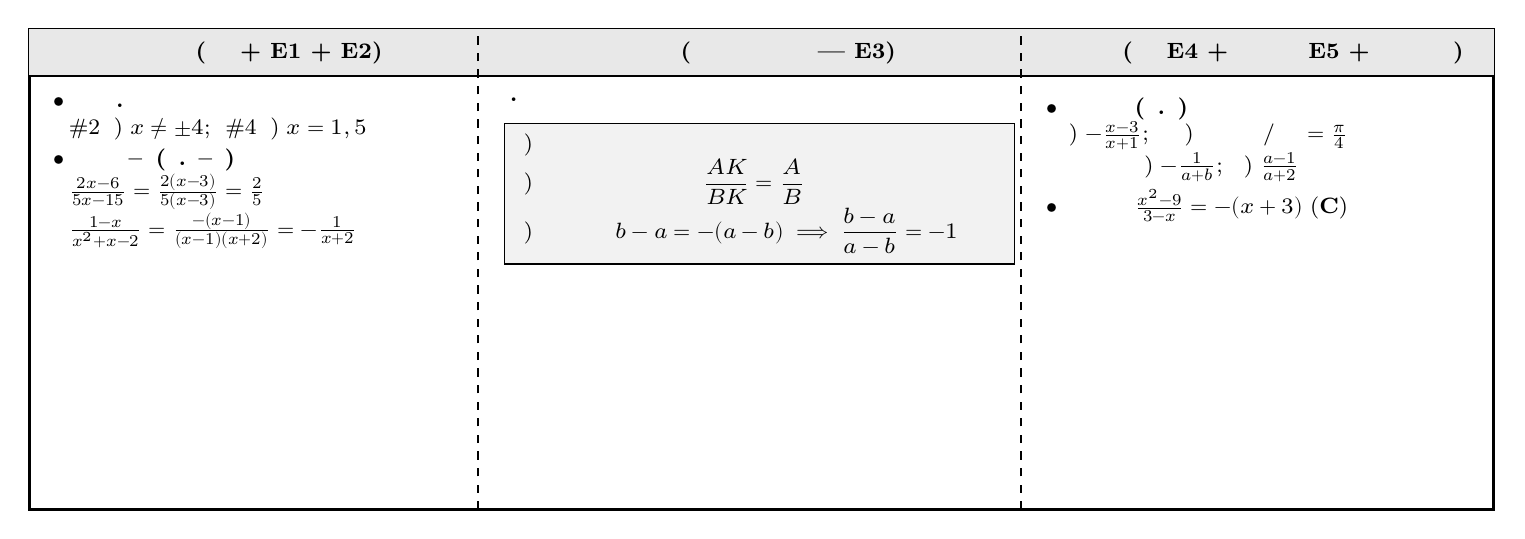
\begin{tikzpicture}[x=1cm, y=1cm, every node/.style={font=\footnotesize, text=black}]
  \draw[black, line width=1.1pt] (0,0) rectangle (18.6,6.1);
  \fill[gray!18] (0,5.50) rectangle (18.6,6.1);
  \draw[black, line width=0.7pt] (0,5.50) -- (18.6,5.50);
  \draw[black, dashed, line width=0.75pt] (5.7,0) -- (5.7,6.1);
  \draw[black, dashed, line width=0.75pt] (12.6,0) -- (12.6,6.1);

  \node at (2.85,5.80) {\textbf{ផ្នែកឆ្វេង (កំណែ + \en{E1} + \en{E2})}};
  \node at (9.15,5.80) {\textbf{ផ្នែកកណ្ដាល (ខ្លឹមសារគោលរក្សាទុក — \en{E3})}};
  \node at (15.60,5.80) {\textbf{ផ្នែកស្ដាំ (គំរូ \en{E4} + ប្រតិបត្តិ \en{E5} + កិច្ចការផ្ទះ)}};

  % Left zone
  \node[anchor=north west, text width=5.3cm] at (0.18,5.35) {
    $\bullet$ \textbf{កំណែ ទំ.៨៥៖}\\
    \hspace*{0.2cm}\en{\#2} ឃ) $x \neq \pm 4$; \ \en{\#4} គ) $x = 1, 5$\\[2pt]
    $\bullet$ \textbf{ឧទាហរណ៍ ១--៤ (ទំ.៧៦--៧៧)៖}\\
    \hspace*{0.2cm}$\tfrac{2x-6}{5x-15} = \tfrac{2(x-3)}{5(x-3)} = \tfrac{2}{5}$\\
    \hspace*{0.2cm}$\tfrac{1-x}{x^2+x-2} = \tfrac{-(x-1)}{(x-1)(x+2)} = -\tfrac{1}{x+2}$
  };

  % Center zone
  \node[anchor=north west, text width=6.5cm] at (5.90,5.35) {
    {\muol\fontsize{8.2pt}{12pt}\selectfont ៣\enbf{.} ការសម្រួលកន្សោមសនិទាន}\\[3pt]
    \begin{tcolorbox}[enhanced, sharp corners, colback=gray!10, colframe=black, boxrule=0.6pt, boxsep=1.5pt, left=3pt, right=3pt, top=2pt, bottom=2pt]
      ១) ដាក់ភាគយកនិងភាគបែងជាផលគុណកត្តាសិន\\
      ២) ចែកនឹងកត្តារួមខុសពីសូន្យ៖ $\dfrac{AK}{BK} = \dfrac{A}{B}$\\
      ៣) កត្តាផ្ទុយ៖ $b - a = -(a - b) \implies \dfrac{b-a}{a-b} = -1$
    \end{tcolorbox}
  };

  % Right zone
  \node[anchor=north west, text width=5.6cm] at (12.80,5.35) {
    $\bullet$ \textbf{លំហាត់គំរូ (ទំ.៧៨)៖}\\
    \hspace*{0.2cm}១) $-\tfrac{x-3}{x+1}$; \quad ២) ផ្ទៃរង្វង់/ការេ $= \tfrac{\pi}{4}$\\
    \hspace*{0.2cm}ប្រតិបត្តិ៖ ក) $-\tfrac{1}{a+b}$; \ ខ) $\tfrac{a-1}{a+2}$\\[2pt]
    $\bullet$ \textbf{វិនិច្ឆ័យ៖} $\tfrac{x^2-9}{3-x} = -(x + 3)$ (\textbf{\en{C}})
  };
\end{tikzpicture}
\end{center}

\secstrip{២. ចម្លើយផ្ទៀងផ្ទាត់រហ័សសម្រាប់សន្លឹកកិច្ចការសិស្ស \enbf{(}ទំព័រ ១ និង ទំព័រ ២\enbf{)}}{\en{Answer Key}}

\begin{tcolorbox}[
  enhanced, sharp corners, colback=white, colframe=black,
  boxrule=0.8pt, boxsep=2.5pt, top=4pt, bottom=4pt, left=6pt, right=6pt
]
  $\bullet$ \textbf{ផ្នែក \en{E1}៖} សិស្ស ខ ត្រឹមត្រូវ (តេស្ត $x=2$៖ សិស្ស ក បាន $-\tfrac{11}{7} \neq 1$; សិស្ស ខ បាន $\tfrac{2}{2} = 1$ ត្រឹមត្រូវ) ។\\[2pt]
  $\bullet$ \textbf{ផ្នែក \en{E2}៖} សកម្មភាព ១៖ $\tfrac{2}{5}$; $\tfrac{4b^2}{5a^3}$ ។ សកម្មភាព ២៖ $\tfrac{x}{3x-4}$; $-\tfrac{1}{x+2}$ ។\\[2pt]
  $\bullet$ \textbf{ផ្នែក \en{E4}៖} ១) $-\tfrac{x-3}{x+1}$; $\tfrac{\pi}{4}$; ២) $-\tfrac{1}{a+b}$; $\tfrac{a-1}{a+2}$ ($a-b = -(b-a)$ ចែកនឹង $b-a$ បាន $-1$) ។\\[2pt]
  $\bullet$ \textbf{ផ្នែក \en{E5}៖} ១) $\tfrac{1}{x+z}$; $\tfrac{a-2}{2(a-3)}$; $\tfrac{2x}{y}$; $\tfrac{1}{2a(x+3)}$; $-(5x+1)$; ២) សិស្ស ខ ($1$); ៣) \textbf{ជម្រើស \en{C}} ($-(x+3)$); ៤) $\tfrac{x+y^2}{y}$ ។
\end{tcolorbox}

\secstrip{៣. ចម្លើយលម្អិតនៃកិច្ចការផ្ទះ \enbf{(}សម្រាប់គ្រូផ្ទៀងផ្ទាត់នៅដើមម៉ោងបន្ទាប់\enbf{)}}{សៀវភៅគោល ទំ.៨៥}

\begin{tcolorbox}[
  enhanced, sharp corners, colback=white, colframe=black,
  boxrule=0.8pt, boxsep=2.5pt, top=4pt, bottom=4pt, left=6pt, right=6pt
]
  $\bullet$ \textbf{១) ទំ.៨៥ \en{\#5} ខ, គ៖} ខ) $\dfrac{-8a^2b^4x}{-8a^3b^3x^3} = \mathbf{\dfrac{b}{ax^2}}$; \quad គ) $\dfrac{x(a-b)^2}{(a-b)^3} = \mathbf{\dfrac{x}{a - b}}$ ។\\[2pt]
  $\bullet$ \textbf{២) ទំ.៨៥ \en{\#5} ដ, ឋ, ឍ៖} ដ) $\dfrac{(a-b)(a-c)}{(a+b)(a-c)} = \mathbf{\dfrac{a-b}{a+b}}$; \ ឋ) $\dfrac{(a-1)(x-y)}{3(x-y)} = \mathbf{\dfrac{a-1}{3}}$; \ ឍ) $\dfrac{(a+6)(a-2)}{(a+4)(a-2)} = \mathbf{\dfrac{a+6}{a+4}}$ ។
\end{tcolorbox}

\end{document}
